\documentclass[11pt]{article}

\usepackage[margin=0.85in]{geometry}
\usepackage[T1]{fontenc}
\usepackage[utf8]{inputenc}
\usepackage{lmodern}
\usepackage{amsmath,amssymb,mathtools}
\usepackage{booktabs}
\usepackage{array}
\usepackage{graphicx}
\usepackage{enumitem}
\usepackage{siunitx}
\usepackage{xcolor}
\usepackage{hyperref}
\usepackage{tikz}
\usepackage{pgfplots}
\usepackage{circuitikz}
\usepackage{tcolorbox}
\usepackage{multicol}
\usepackage{longtable}
\usetikzlibrary{arrows.meta,positioning,calc,shapes.geometric,fit}
\pgfplotsset{compat=1.18}

\hypersetup{
  colorlinks=true,
  linkcolor=blue!55!black,
  urlcolor=blue!55!black,
  citecolor=blue!55!black
}

\newcommand{\V}{\mathbf{V}}
\newcommand{\I}{\mathbf{I}}
\newcommand{\Y}{\mathbf{Y}}
\newcommand{\Sbase}{S_{\mathrm{base}}}
\newcommand{\Vbase}{V_{\mathrm{base}}}
\newcommand{\Zbase}{Z_{\mathrm{base}}}
\newcommand{\pu}{\mathrm{pu}}
\newcommand{\dd}{\mathrm{d}}
\newcommand{\junit}{\mathrm{j}}
\newcommand{\Real}{\operatorname{Re}}
\newcommand{\Imag}{\operatorname{Im}}
\newcommand{\highlight}[1]{\textcolor{blue!55!black}{#1}}

\title{\textbf{Power System Study Guide}\\
\large From Classical Network Analysis to Inverter-Based Resources, Grid-Forming Control, and Microgrid Fault Ride-Through}
\author{Generated Study Notes}
\date{\today}

\begin{document}
\maketitle

\begin{abstract}
This guide summarizes core and advanced power-system topics: per-unit
normalization, bus modeling, power-flow equations, voltage and angle stability,
faults, protection, synchronous-machine dynamics, inverter-based resources
(IBRs), grid-following (GFL) and grid-forming (GFM) controls, the stability
impact of high IBR penetration, and practical ride-through concepts for
microgrids during grid faults. Equations and figures are included to make the
material useful as both a review sheet and an implementation reference.
\end{abstract}

\tableofcontents
\newpage

\section{Big Picture}

An electric power system converts mechanical, chemical, solar, wind, or stored
energy into electric power, transports it through transmission and distribution
networks, and delivers it to loads with acceptable voltage, frequency,
reliability, power quality, and safety. The traditional grid is dominated by
synchronous generators. Modern grids increasingly include inverter-based
resources such as wind, solar photovoltaic (PV), battery energy storage systems
(BESS), and power-electronic loads.

\begin{figure}[h]
\centering
\resizebox{0.95\linewidth}{!}{%
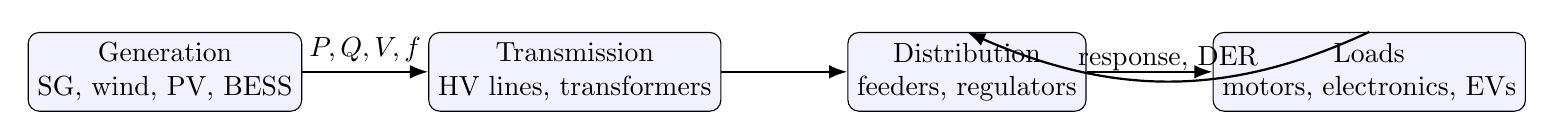
\begin{tikzpicture}[node distance=1.6cm,>=Latex]
  \tikzstyle{block}=[draw,rounded corners,align=center,minimum width=2.6cm,minimum height=1.0cm,fill=blue!5]
  \node[block] (gen) {Generation\\SG, wind, PV, BESS};
  \node[block,right=of gen] (tx) {Transmission\\HV lines, transformers};
  \node[block,right=of tx] (dist) {Distribution\\feeders, regulators};
  \node[block,right=of dist] (load) {Loads\\motors, electronics, EVs};
  \draw[->,thick] (gen) -- node[above] {$P,Q,V,f$} (tx);
  \draw[->,thick] (tx) -- (dist);
  \draw[->,thick] (dist) -- (load);
  \draw[->,thick,bend left=25] (load.north) to node[above] {response, DER} (dist.north);
\end{tikzpicture}
}
\caption{A power system is a controlled energy-conversion network.}
\end{figure}

\section{Phasors, Complex Power, and Per-Unit}

\subsection{Sinusoidal Steady State}
For a sinusoidal voltage,
\begin{equation}
v(t)=\sqrt{2}V_{\mathrm{rms}}\cos(\omega t+\theta),
\end{equation}
the phasor is
\begin{equation}
\tilde{V}=V_{\mathrm{rms}}\angle\theta.
\end{equation}
For balanced three-phase systems, a single-phase equivalent is commonly used.
Line-to-line and phase quantities obey
\begin{equation}
V_{LL}=\sqrt{3}V_{\phi}, \qquad S_{3\phi}=\sqrt{3}V_{LL}I_L.
\end{equation}

\subsection{Complex Power}
Complex power is
\begin{equation}
\tilde{S}=P+\junit Q=\tilde{V}\tilde{I}^{*},
\end{equation}
where $P$ is real power and $Q$ is reactive power. The power factor is
\begin{equation}
\mathrm{pf}=\cos\phi=\frac{P}{|\tilde{S}|}.
\end{equation}
For inductive loads, current lags voltage and $Q>0$ under the usual load sign
convention.

\subsection{Per-Unit System}
Per-unit quantities reduce transformer-ratio bookkeeping and put impedances on
a comparable scale:
\begin{equation}
X_{\pu}=\frac{X_{\mathrm{actual}}}{X_{\mathrm{base}}}.
\end{equation}
For a three-phase base,
\begin{equation}
Z_{\mathrm{base}}=\frac{V_{LL,\mathrm{base}}^2}{S_{3\phi,\mathrm{base}}},
\qquad
I_{\mathrm{base}}=\frac{S_{3\phi,\mathrm{base}}}{\sqrt{3}V_{LL,\mathrm{base}}}.
\end{equation}
Changing base:
\begin{equation}
Z_{\pu,\mathrm{new}}=Z_{\pu,\mathrm{old}}
\left(\frac{S_{\mathrm{base,new}}}{S_{\mathrm{base,old}}}\right)
\left(\frac{V_{\mathrm{base,old}}}{V_{\mathrm{base,new}}}\right)^2.
\end{equation}

\section{Network Modeling}

\subsection{Transmission-Line Models}
For a short line, shunt capacitance can often be neglected:
\begin{equation}
\tilde{V}_S=\tilde{V}_R+\tilde{I}(R+\junit X).
\end{equation}
For medium and long lines, the nominal-$\pi$ model includes shunt admittance
$Y/2$ at both ends.

\begin{figure}[h]
\centering
\begin{circuitikz}[american]
\draw (0,0) to[short,o-] (1,0)
      to[R=$R$, -*] (3,0)
      to[L=$X/\omega$, -*] (5,0)
      to[short,-o] (6,0);
\draw (1,0) to[C,l_=$Y/2\omega$] (1,-2) node[ground]{};
\draw (5,0) to[C,l=$Y/2\omega$] (5,-2) node[ground]{};
\node at (0,0.35) {$V_S$};
\node at (6,0.35) {$V_R$};
\end{circuitikz}
\caption{Nominal-$\pi$ transmission-line model.}
\end{figure}

\subsection{Admittance Matrix}
Nodal current injection satisfies
\begin{equation}
\I=\Y_{\mathrm{bus}}\V.
\end{equation}
For a branch between buses $i$ and $k$ with series admittance $y_{ik}$:
\begin{align}
Y_{ii} &\leftarrow Y_{ii}+y_{ik}+y_{\mathrm{sh},i},\\
Y_{kk} &\leftarrow Y_{kk}+y_{ik}+y_{\mathrm{sh},k},\\
Y_{ik} &=Y_{ki}\leftarrow -y_{ik}.
\end{align}
Transformer off-nominal tap ratios and phase shifters modify these entries and
must be modeled carefully in power-flow and short-circuit studies.

\section{Bus Types: Slack, PV, and PQ}

Power-flow analysis classifies buses by which variables are specified and which
are solved.

\begin{table}[h]
\centering
\begin{tabular}{llll}
\toprule
Bus type & Known quantities & Unknown quantities & Typical device \\
\midrule
Slack / swing & $|V|,\delta$ & $P,Q$ & Reference generator \\
PV / generator & $P,|V|$ & $Q,\delta$ & Generator with AVR \\
PQ / load & $P,Q$ & $|V|,\delta$ & Load or fixed-power DER \\
\bottomrule
\end{tabular}
\caption{Power-flow bus types.}
\end{table}

\begin{itemize}
  \item \textbf{Slack bus:} supplies the real and reactive mismatch after all
  other injections and losses are determined. It sets the system angle reference.
  \item \textbf{PV bus:} real power and voltage magnitude are specified. Reactive
  output is solved, but if it violates limits, the bus is typically converted to
  PQ with $Q$ fixed at the limit.
  \item \textbf{PQ bus:} real and reactive powers are specified. Voltage magnitude
  and angle are solved.
\end{itemize}

\begin{figure}[h]
\centering
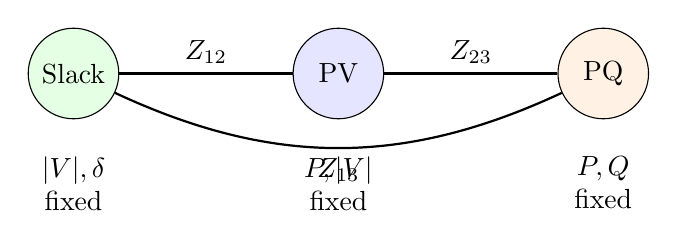
\begin{tikzpicture}[node distance=2.2cm,>=Latex]
  \node[draw,circle,fill=green!10,minimum size=1.15cm] (slack) {Slack};
  \node[draw,circle,fill=blue!10,minimum size=1.15cm,right=of slack] (pv) {PV};
  \node[draw,circle,fill=orange!10,minimum size=1.15cm,right=of pv] (pq) {PQ};
  \draw[thick] (slack) -- node[above] {$Z_{12}$} (pv);
  \draw[thick] (pv) -- node[above] {$Z_{23}$} (pq);
  \draw[thick,bend right=25] (slack) to node[below] {$Z_{13}$} (pq);
  \node[below=0.35cm of slack,align=center] {$|V|,\delta$\\fixed};
  \node[below=0.35cm of pv,align=center] {$P,|V|$\\fixed};
  \node[below=0.35cm of pq,align=center] {$P,Q$\\fixed};
\end{tikzpicture}
\caption{Three classical power-flow bus types.}
\end{figure}

\section{AC Power Flow}

\subsection{Power Injection Equations}
Let $V_i=|V_i|\angle\delta_i$ and
$Y_{ik}=G_{ik}+\junit B_{ik}$. The complex power injected at bus $i$ is
\begin{equation}
S_i=P_i+\junit Q_i=V_i I_i^*=V_i\left(\sum_{k=1}^{n}Y_{ik}V_k\right)^*.
\end{equation}
The real and reactive power equations are
\begin{align}
P_i &= |V_i|\sum_{k=1}^{n}|V_k|
\left(G_{ik}\cos\delta_{ik}+B_{ik}\sin\delta_{ik}\right),\\
Q_i &= |V_i|\sum_{k=1}^{n}|V_k|
\left(G_{ik}\sin\delta_{ik}-B_{ik}\cos\delta_{ik}\right),
\end{align}
where $\delta_{ik}=\delta_i-\delta_k$.

\subsection{Newton--Raphson Method}
Define mismatch vector
\begin{equation}
\Delta x=
\begin{bmatrix}
\Delta P\\
\Delta Q
\end{bmatrix}
=
\begin{bmatrix}
P_{\mathrm{spec}}-P_{\mathrm{calc}}\\
Q_{\mathrm{spec}}-Q_{\mathrm{calc}}
\end{bmatrix}.
\end{equation}
At iteration $r$,
\begin{equation}
\begin{bmatrix}
\Delta P\\
\Delta Q
\end{bmatrix}^{(r)}
=
\begin{bmatrix}
H & N\\
M & L
\end{bmatrix}^{(r)}
\begin{bmatrix}
\Delta \delta\\
\Delta |V|
\end{bmatrix}^{(r)}.
\end{equation}
Update angles and magnitudes until the maximum mismatch is below tolerance.

\subsection{Fast Decoupled Power Flow}
For high-voltage transmission systems, $X\gg R$, voltage magnitudes are near
1 pu, and angle differences are small. Then active power is strongly coupled to
angle and reactive power to voltage:
\begin{align}
\Delta P/|V| &\approx B'\Delta \delta,\\
\Delta Q/|V| &\approx B''\Delta |V|.
\end{align}

\section{Economic Dispatch and Optimal Power Flow}

\subsection{Economic Dispatch}
For generator cost
\begin{equation}
C_i(P_i)=a_iP_i^2+b_iP_i+c_i,
\end{equation}
economic dispatch without losses solves
\begin{equation}
\min_{P_i}\sum_i C_i(P_i)
\quad \text{s.t.}\quad
\sum_i P_i=P_D.
\end{equation}
The optimality condition is
\begin{equation}
\frac{\dd C_i}{\dd P_i}=2a_iP_i+b_i=\lambda,
\end{equation}
subject to generator limits.

\subsection{AC Optimal Power Flow}
AC OPF extends power flow by optimizing an objective subject to network
constraints:
\begin{align}
\min_{V,\delta,P_G,Q_G} \quad & f(P_G,Q_G,V)\\
\text{s.t.}\quad & g(V,\delta,P_G,Q_G)=0,\\
& h(V,\delta,P_G,Q_G)\le 0.
\end{align}
Constraints include bus voltage limits, branch thermal limits, generator
capability curves, reserve requirements, and security constraints.

\section{Short-Circuit and Fault Analysis}

\subsection{Symmetrical Components}
Unbalanced three-phase quantities can be decomposed into positive, negative,
and zero sequences:
\begin{equation}
\begin{bmatrix}V_a\\V_b\\V_c\end{bmatrix}
=
\begin{bmatrix}
1&1&1\\
1&a^2&a\\
1&a&a^2
\end{bmatrix}
\begin{bmatrix}V_0\\V_1\\V_2\end{bmatrix},
\qquad
a=e^{\junit 2\pi/3}.
\end{equation}
The inverse transform is
\begin{equation}
\begin{bmatrix}V_0\\V_1\\V_2\end{bmatrix}
=\frac{1}{3}
\begin{bmatrix}
1&1&1\\
1&a&a^2\\
1&a^2&a
\end{bmatrix}
\begin{bmatrix}V_a\\V_b\\V_c\end{bmatrix}.
\end{equation}

\subsection{Three-Phase Fault}
For a bolted balanced three-phase fault at a bus with Thevenin voltage
$V_{\mathrm{th}}$ and Thevenin impedance $Z_1$,
\begin{equation}
I_f=\frac{V_{\mathrm{th}}}{Z_1+Z_f}.
\end{equation}

\subsection{Single-Line-to-Ground Fault}
For an $a$-phase-to-ground fault:
\begin{equation}
I_a=3I_0=\frac{3V_{\mathrm{th}}}{Z_1+Z_2+Z_0+3Z_f}.
\end{equation}
Grounding and transformer connections strongly affect $Z_0$ and therefore
ground-fault current.

\subsection{Fault Current From Synchronous Machines and IBRs}
Synchronous generators can contribute large transient currents, often several
per-unit initially, limited by subtransient reactance:
\begin{equation}
I_{\mathrm{sc,SG}}\approx \frac{E''}{X''_d}.
\end{equation}
IBRs are current-limited by semiconductors and controls, commonly around
$1.1$--$2.0$ pu depending on design and grid code:
\begin{equation}
|\tilde{I}_{\mathrm{IBR}}|\le I_{\max}.
\end{equation}
This changes protection sensitivity, directionality, relay coordination, and
fault-location methods.

\section{Protection Fundamentals}

Protection detects abnormal conditions and isolates faulted equipment quickly.
Common functions include:
\begin{itemize}
  \item \textbf{50/51 overcurrent:} instantaneous/time-delayed current pickup.
  \item \textbf{67 directional overcurrent:} uses voltage polarization to infer
  fault direction.
  \item \textbf{21 distance:} estimates apparent impedance $Z_{\mathrm{app}}=V/I$.
  \item \textbf{87 differential:} compares currents entering and leaving a zone.
  \item \textbf{27/59 undervoltage/overvoltage} and \textbf{81U/O frequency}
  functions.
  \item \textbf{ROCOF:} rate-of-change-of-frequency, $\dd f/\dd t$.
\end{itemize}

\begin{tcolorbox}[colback=yellow!6,colframe=yellow!45!black,title=IBR Protection Challenge]
High IBR penetration reduces short-circuit current magnitude, changes current
phase angle through control actions, and can make conventional overcurrent
protection less dependable. Protection may need adaptive settings, negative-
sequence quantities, differential schemes, transfer trip, traveling waves, or
communications-assisted logic.
\end{tcolorbox}

\section{Voltage Control and Reactive Power}

\subsection{Reactive Power and Voltage}
In transmission networks with $X\gg R$, reactive power strongly affects voltage.
A useful approximate relation is
\begin{equation}
\Delta V\approx \frac{XQ+RP}{V}.
\end{equation}
Devices for voltage support include generator automatic voltage regulators
(AVRs), shunt capacitors/reactors, static VAR compensators (SVC), STATCOMs,
load tap changers, and inverter volt-var controls.

\subsection{Generator Capability}
Synchronous-generator reactive power is limited by armature current, field
current, end-region heating, and stability. IBR reactive capability is limited
by current and dc-link constraints:
\begin{equation}
P^2+Q^2\le S_{\mathrm{rated}}^2, \qquad
I_d^2+I_q^2\le I_{\max}^2.
\end{equation}
During faults, priority may be given to reactive current injection:
\begin{equation}
I_q^{*}=k_{\mathrm{FRT}}\left(V_{\mathrm{ref}}-V_{\mathrm{PCC}}\right),
\qquad |I^*|\le I_{\max}.
\end{equation}

\section{Frequency Control and Inertia}

\subsection{Swing Equation}
The synchronous-machine rotor angle follows
\begin{equation}
M\frac{\dd^2\delta}{\dd t^2}=P_m-P_e-D\frac{\dd \delta}{\dd t},
\end{equation}
or, in frequency form,
\begin{equation}
\frac{2H}{f_0}\frac{\dd f}{\dd t}=P_m-P_e-D_f(f-f_0),
\end{equation}
where $H$ is the inertia constant. Immediately after a generation-loss event,
frequency rate of change is approximately
\begin{equation}
\frac{\dd f}{\dd t}\approx \frac{f_0}{2H_{\mathrm{sys}}}
\left(\frac{\Delta P}{S_{\mathrm{base}}}\right).
\end{equation}

\subsection{Primary, Secondary, and Tertiary Control}
\begin{itemize}
  \item \textbf{Primary control:} governor or inverter droop responds in seconds.
  \item \textbf{Secondary control:} automatic generation control restores
  frequency and tie-line interchange in tens of seconds to minutes.
  \item \textbf{Tertiary control:} economic redispatch and reserve management.
\end{itemize}

\section{Stability Concepts}

\subsection{Rotor-Angle Stability}
Rotor-angle stability is the ability of synchronous machines to remain in
synchronism. For a classical generator connected to an infinite bus:
\begin{equation}
P_e=\frac{EV}{X}\sin\delta.
\end{equation}
The synchronizing torque coefficient is
\begin{equation}
K_s=\frac{\partial P_e}{\partial \delta}=\frac{EV}{X}\cos\delta.
\end{equation}
As $\delta$ approaches \SI{90}{\degree}, synchronizing torque decreases.

\subsection{Equal-Area Criterion}
For a single-machine infinite-bus system, transient stability can be assessed by
comparing accelerating and decelerating areas on the $P$--$\delta$ curve:
\begin{equation}
A_{\mathrm{acc}}=\int_{\delta_0}^{\delta_c}(P_m-P_{e,\mathrm{fault}})\,\dd\delta,
\qquad
A_{\mathrm{dec}}=\int_{\delta_c}^{\delta_{\max}}(P_{e,\mathrm{post}}-P_m)\,\dd\delta.
\end{equation}
Stability requires $A_{\mathrm{dec}}\ge A_{\mathrm{acc}}$.

\subsection{Voltage Stability}
Voltage stability is the ability to maintain acceptable voltage after a
disturbance. A simple radial two-bus example shows the ``nose curve'':

\begin{figure}[h]
\centering
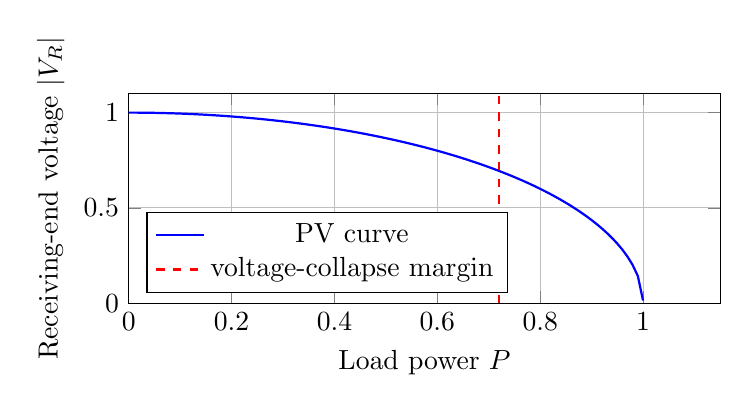
\begin{tikzpicture}
\begin{axis}[
  width=0.75\linewidth,
  height=0.35\linewidth,
  xlabel={Load power $P$},
  ylabel={Receiving-end voltage $|V_R|$},
  xmin=0,xmax=1.15,ymin=0,ymax=1.1,
  grid=both,
  domain=0:1,
  samples=100,
  legend style={at={(0.03,0.05)},anchor=south west}
]
\addplot[blue,thick] ({x},{sqrt(max(0,1-x^2))});
\addplot[red,dashed,thick] coordinates {(0.72,0) (0.72,1.1)};
\legend{PV curve, voltage-collapse margin}
\end{axis}
\end{tikzpicture}
\caption{Conceptual PV curve showing maximum loadability and voltage-collapse margin.}
\end{figure}

\subsection{Small-Signal Stability}
Linearize nonlinear dynamics $\dot{x}=f(x,u)$ around an operating point:
\begin{equation}
\Delta \dot{x}=A\Delta x+B\Delta u.
\end{equation}
Eigenvalues $\lambda_i=\sigma_i+\junit \omega_i$ determine modal behavior.
The damping ratio is
\begin{equation}
\zeta_i=\frac{-\sigma_i}{\sqrt{\sigma_i^2+\omega_i^2}}.
\end{equation}
Negative damping or weak inter-area modes can be worsened by controls that
interact with grid impedance, PLLs, or other converters.

\section{Power Quality}

Power quality includes voltage sags, swells, interruptions, harmonics, flicker,
unbalance, and transients. Harmonic distortion is quantified by
\begin{equation}
\mathrm{THD}_V=\frac{\sqrt{V_2^2+V_3^2+\cdots+V_n^2}}{V_1}.
\end{equation}
Converters use filters and controls to meet harmonic limits. Resonance can occur
when inverter filters, cable capacitance, transformer leakage, and grid
impedance form lightly damped modes.

\section{Inverter-Based Resources}

\subsection{What Is an IBR?}
An IBR interfaces an energy source or storage device through power electronics.
Examples include PV inverters, wind turbine full converters, type-3 wind
generators with partial converters, BESS, fuel cells, and many HVDC terminals.

\subsection{Converter Power Equations in $dq$ Coordinates}
With the $d$-axis aligned to voltage, $v_q=0$:
\begin{align}
P &= \frac{3}{2}(v_di_d+v_qi_q)=\frac{3}{2}v_di_d,\\
Q &= \frac{3}{2}(v_qi_d-v_di_q)=-\frac{3}{2}v_di_q.
\end{align}
Thus $i_d$ controls active power and $i_q$ controls reactive power under this
axis convention.

\subsection{Grid-Following (GFL) Inverters}
A GFL inverter behaves like a controlled current source. It synchronizes to an
existing grid voltage using a phase-locked loop (PLL), then injects commanded
currents.

\begin{figure}[h]
\centering
\resizebox{0.95\linewidth}{!}{%
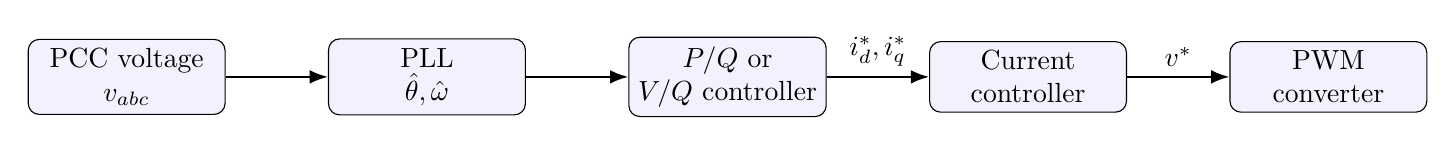
\begin{tikzpicture}[>=Latex,node distance=1.3cm]
  \tikzstyle{block}=[draw,rounded corners,align=center,minimum width=2.5cm,minimum height=0.8cm,fill=blue!5]
  \node[block] (pcc) {PCC voltage\\$v_{abc}$};
  \node[block,right=of pcc] (pll) {PLL\\$\hat{\theta},\hat{\omega}$};
  \node[block,right=of pll] (pq) {$P/Q$ or\\$V/Q$ controller};
  \node[block,right=of pq] (curr) {Current\\controller};
  \node[block,right=of curr] (pwm) {PWM\\converter};
  \draw[->,thick] (pcc) -- (pll);
  \draw[->,thick] (pll) -- (pq);
  \draw[->,thick] (pq) -- node[above] {$i_d^*,i_q^*$} (curr);
  \draw[->,thick] (curr) -- node[above] {$v^*$} (pwm);
\end{tikzpicture}
}
\caption{Grid-following inverter control is synchronized by the measured grid voltage.}
\end{figure}

Typical GFL PLL dynamics include
\begin{equation}
\dot{\hat{\theta}}=\omega_0+K_p v_q+K_i\int v_q\,\dd t.
\end{equation}
GFL inverters are effective in strong grids but can struggle in weak grids or
islanded microgrids because they require a voltage reference to follow.

\subsection{Grid-Forming (GFM) Inverters}
A GFM inverter behaves more like a controllable voltage source behind an
impedance. It establishes voltage magnitude and frequency rather than relying
entirely on an external voltage.

Common GFM approaches:
\begin{itemize}
  \item \textbf{Droop control:}
  \begin{align}
  \omega &= \omega_0-m_p(P-P_0),\\
  V &= V_0-n_q(Q-Q_0).
  \end{align}
  \item \textbf{Virtual synchronous machine (VSM):}
  \begin{equation}
  2H_{\mathrm{v}}\dot{\omega}=P^{*}-P-D_{\mathrm{v}}(\omega-\omega_0).
  \end{equation}
  \item \textbf{Dispatchable virtual oscillator control:} nonlinear oscillator
  dynamics regulate voltage waveform and share power.
  \item \textbf{Matching control:} uses dc-link dynamics to emulate
  synchronous-machine electromechanical coupling.
\end{itemize}

\begin{figure}[h]
\centering
\resizebox{0.95\linewidth}{!}{%
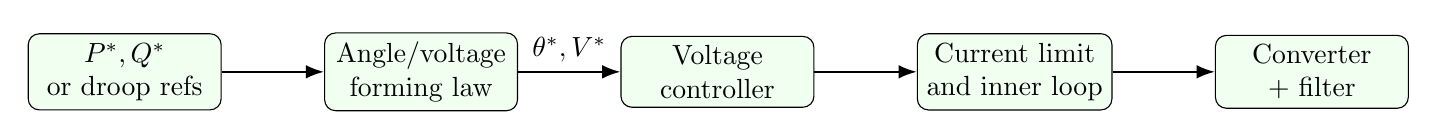
\begin{tikzpicture}[>=Latex,node distance=1.3cm]
  \tikzstyle{block}=[draw,rounded corners,align=center,minimum width=2.45cm,minimum height=0.8cm,fill=green!6]
  \node[block] (pref) {$P^*,Q^*$\\or droop refs};
  \node[block,right=of pref] (osc) {Angle/voltage\\forming law};
  \node[block,right=of osc] (volt) {Voltage\\controller};
  \node[block,right=of volt] (curr) {Current limit\\and inner loop};
  \node[block,right=of curr] (conv) {Converter\\+ filter};
  \draw[->,thick] (pref) -- (osc);
  \draw[->,thick] (osc) -- node[above] {$\theta^*,V^*$} (volt);
  \draw[->,thick] (volt) -- (curr);
  \draw[->,thick] (curr) -- (conv);
\end{tikzpicture}
}
\caption{Grid-forming inverter control creates a voltage/frequency reference.}
\end{figure}

\subsection{GFL vs GFM Summary}
\begin{longtable}{p{0.2\linewidth}p{0.36\linewidth}p{0.36\linewidth}}
\toprule
Feature & Grid-following & Grid-forming \\
\midrule
Equivalent behavior & Current source & Voltage source behind impedance \\
Synchronization & PLL follows grid voltage & Internal oscillator or swing-like law \\
Islanded operation & Not sufficient alone & Can support islanded microgrid \\
Weak-grid performance & PLL/control interactions possible & Can improve voltage/frequency stiffness \\
Fault response & Current-limited injection & Must handle current limiting without losing voltage-forming behavior \\
Power sharing & Usually outer-loop command & Droop/VSM sharing natural \\
\bottomrule
\end{longtable}

\section{How IBRs Affect Power-Grid Stability}

\subsection{Reduced Inertia and Faster Dynamics}
Replacing synchronous machines with IBRs reduces physical rotating inertia unless
the IBR control intentionally provides synthetic inertia or fast frequency
response. Lower inertia produces higher ROCOF:
\begin{equation}
\left|\frac{\dd f}{\dd t}\right|\propto \frac{|\Delta P|}{H_{\mathrm{sys}}}.
\end{equation}
However, IBRs can respond much faster than mechanical governors if controls,
energy headroom, and communications are designed correctly.

\subsection{PLL and Weak-Grid Instability}
Grid strength is often measured using short-circuit ratio:
\begin{equation}
\mathrm{SCR}=\frac{S_{\mathrm{sc}}}{S_{\mathrm{IBR,rated}}},
\qquad
S_{\mathrm{sc}}=\frac{V^2}{|Z_{\mathrm{th}}|}.
\end{equation}
Low SCR means the inverter's own current injection significantly moves the PCC
voltage. For GFL controls, PLL dynamics can couple with the weak grid and create
oscillations. Effective grid strength can also be reduced by nearby converters
interacting through the same network.

\subsection{Current Limiting and Protection}
IBRs cannot supply unlimited fault current. During severe voltage depressions,
the current limit
\begin{equation}
\sqrt{i_d^2+i_q^2}\le I_{\max}
\end{equation}
forces a choice between active current, reactive support, negative-sequence
current, and dc-link protection. This affects voltage recovery, relay
dependability, and transient stability.

\subsection{Control Interactions}
High IBR penetration introduces many fast controls: PLLs, current loops, dc-link
loops, volt-var controls, plant-level controllers, and grid-forming controllers.
Interactions can occur over milliseconds to seconds. Stability studies must
include electromagnetic transient (EMT) simulations for fast converter controls
when RMS phasor models are insufficient.

\subsection{Fault-Induced Delayed Voltage Recovery}
IBRs often ride through voltage sags and inject reactive current, but motor loads,
feeder controls, and current-limited converters may cause slow voltage recovery.
Coordination among DER ride-through, distribution protection, and transmission
voltage controls is essential.

\section{Microgrids}

\subsection{Definition and Modes}
A microgrid is a local system of loads, DERs, storage, protection, and controls
that can operate grid-connected or islanded. It needs:
\begin{itemize}
  \item at least one grid-forming source for islanded voltage/frequency,
  \item energy management for power balance,
  \item protection that works for both grid-connected and islanded fault levels,
  \item black-start and resynchronization procedures.
\end{itemize}

\subsection{Microgrid Control Hierarchy}
\begin{enumerate}
  \item \textbf{Primary control:} local voltage/frequency regulation, droop,
  current limiting, and virtual impedance.
  \item \textbf{Secondary control:} restores frequency/voltage deviations caused
  by droop and coordinates multiple DERs.
  \item \textbf{Tertiary control:} economic dispatch and power exchange with the
  main grid.
\end{enumerate}

\begin{figure}[h]
\centering
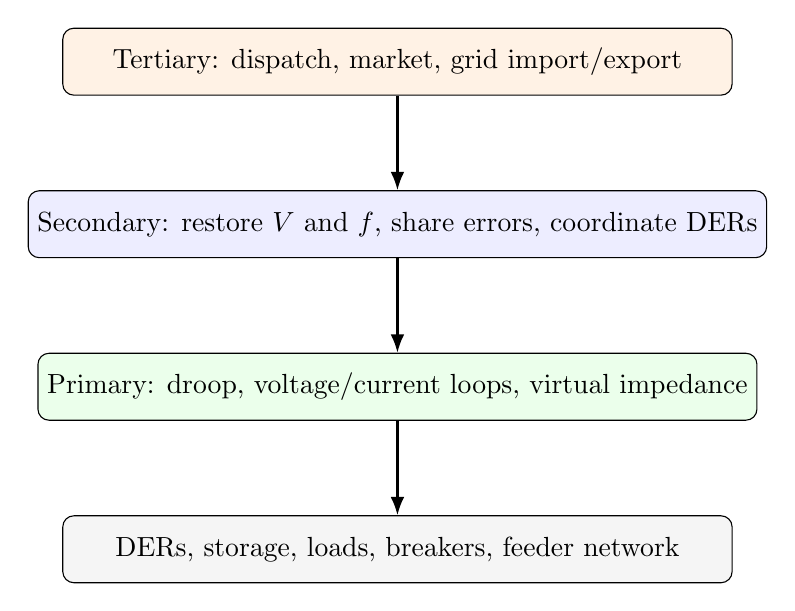
\begin{tikzpicture}[>=Latex,node distance=1.2cm]
  \tikzstyle{layer}=[draw,rounded corners,align=center,minimum width=8.5cm,minimum height=0.85cm]
  \node[layer,fill=green!8] (primary) {Primary: droop, voltage/current loops, virtual impedance};
  \node[layer,fill=blue!7,above=of primary] (secondary) {Secondary: restore $V$ and $f$, share errors, coordinate DERs};
  \node[layer,fill=orange!10,above=of secondary] (tertiary) {Tertiary: dispatch, market, grid import/export};
  \draw[->,thick] (tertiary) -- (secondary);
  \draw[->,thick] (secondary) -- (primary);
  \node[draw,rounded corners,fill=gray!8,below=of primary,minimum width=8.5cm,minimum height=0.85cm,align=center] (plant)
  {DERs, storage, loads, breakers, feeder network};
  \draw[->,thick] (primary) -- (plant);
\end{tikzpicture}
\caption{Microgrid hierarchical control.}
\end{figure}

\section{Ride-Through During Faults}

\subsection{Meaning of Ride-Through}
Ride-through means that DERs remain connected and support the grid or microgrid
during abnormal voltage/frequency events instead of tripping immediately.
Requirements are usually defined by voltage--time and frequency--time envelopes.

\begin{figure}[h]
\centering
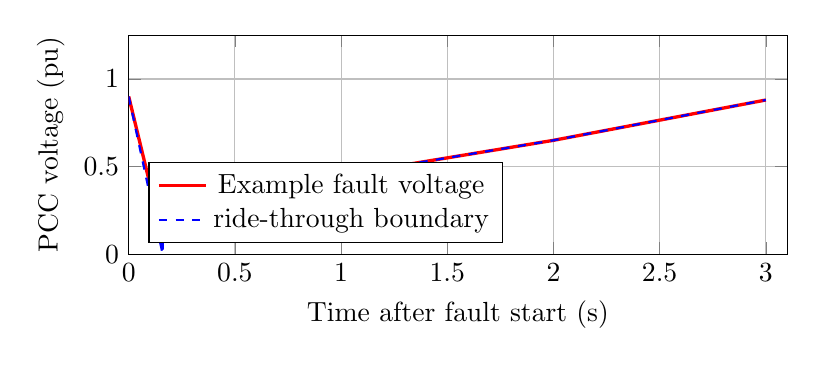
\begin{tikzpicture}
\begin{axis}[
  width=0.82\linewidth,
  height=0.36\linewidth,
  xlabel={Time after fault start (s)},
  ylabel={PCC voltage (pu)},
  xmin=0,xmax=3.1,ymin=0,ymax=1.25,
  grid=both,
  legend style={at={(0.03,0.05)},anchor=south west}
]
\addplot[red,very thick] coordinates {(0,0.9) (0.15,0.15) (0.625,0.15) (1.0,0.45) (2.0,0.65) (3.0,0.88)};
\addplot[blue,dashed,thick] coordinates {(0,0.9) (0.16,0.0) (0.16,0.45) (1.0,0.45) (2.0,0.65) (3.0,0.88)};
\legend{Example fault voltage, ride-through boundary}
\end{axis}
\end{tikzpicture}
\caption{Conceptual low-voltage ride-through envelope. Actual limits depend on grid code.}
\end{figure}

\subsection{Core Ride-Through Mechanisms}
Fault ride-through for an inverter-dominated microgrid usually combines:
\begin{enumerate}
  \item \textbf{Fast fault detection:} voltage sag, current rise, negative/zero
  sequence, impedance, or differential signals.
  \item \textbf{Current limiting:} protects semiconductors and filters while
  maintaining a controlled current vector.
  \item \textbf{Reactive current priority:} supports voltage at the PCC during
  low-voltage events.
  \item \textbf{Active power reduction:} prevents dc-link overvoltage when ac
  power export is limited by sagged voltage.
  \item \textbf{Energy buffering:} BESS, dc-link capacitance, braking chopper, or
  curtailment absorbs mismatch.
  \item \textbf{Protection coordination:} isolates only the faulted zone.
  \item \textbf{Post-fault recovery:} ramps current, voltage, and power references
  to avoid secondary dips or converter interactions.
\end{enumerate}

\subsection{Current-Limited Control During a Fault}
Let $I_{\max}$ be the converter current limit. A common current-priority logic is
\begin{align}
i_q^{*} &= \operatorname{sat}\left(k_v(V_{\mathrm{ref}}-V_{\mathrm{PCC}}),
 -I_{\max}, I_{\max}\right),\\
i_d^{*} &= \operatorname{sgn}(P^{*})
\sqrt{\max\left(I_{\max}^2-(i_q^{*})^2,0\right)}.
\end{align}
If the inverter uses the opposite $dq$ sign convention, the sign of $i_q$ must be
changed. For GFM inverters, the current limit must be integrated without abruptly
collapsing the voltage reference. Common methods are virtual impedance, voltage
reference saturation, current reference limiting, and mode switching to a
protected current-source behavior.

\subsection{GFM Fault Ride-Through}
GFM ride-through is difficult because a voltage source behind low impedance would
naturally produce very high fault current. Practical GFM controls add a virtual
impedance:
\begin{equation}
v_{\mathrm{cmd}}=v_{\mathrm{gfm}}-R_v i-L_v\frac{\dd i}{\dd t},
\end{equation}
or reduce voltage reference when current approaches the limit:
\begin{equation}
V^{*}_{\mathrm{lim}}=V^{*}\min\left(1,\frac{I_{\max}}{|I|}\right).
\end{equation}
After clearing, the controller restores normal voltage-forming behavior with
rate limits:
\begin{equation}
\left|\frac{\dd P^{*}}{\dd t}\right|\le r_P,\qquad
\left|\frac{\dd V^{*}}{\dd t}\right|\le r_V.
\end{equation}

\subsection{Microgrid Fault-Ride-Through Sequence}
\begin{figure}[h]
\centering
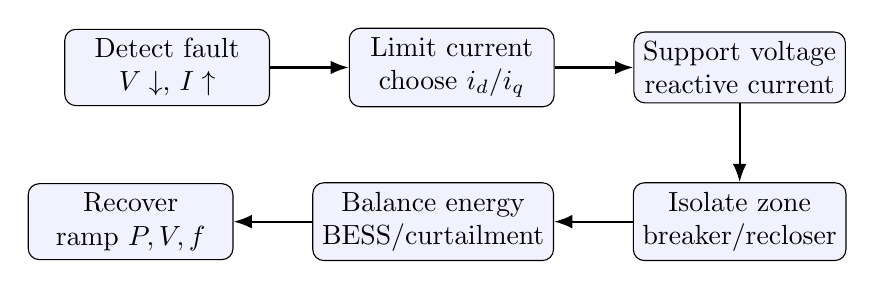
\begin{tikzpicture}[>=Latex,node distance=1.0cm]
  \tikzstyle{rtstep}=[draw,rounded corners,align=center,minimum width=2.6cm,minimum height=0.8cm,fill=blue!5]
  \node[rtstep] (detect) {Detect fault\\$V\downarrow$, $I\uparrow$};
  \node[rtstep,right=of detect] (limit) {Limit current\\choose $i_d/i_q$};
  \node[rtstep,right=of limit] (support) {Support voltage\\reactive current};
  \node[rtstep,below=of support] (isolate) {Isolate zone\\breaker/recloser};
  \node[rtstep,left=of isolate] (balance) {Balance energy\\BESS/curtailment};
  \node[rtstep,left=of balance] (recover) {Recover\\ramp $P,V,f$};
  \draw[->,thick] (detect) -- (limit);
  \draw[->,thick] (limit) -- (support);
  \draw[->,thick] (support) -- (isolate);
  \draw[->,thick] (isolate) -- (balance);
  \draw[->,thick] (balance) -- (recover);
\end{tikzpicture}
\caption{A practical sequence for microgrid fault ride-through.}
\end{figure}

\subsection{Islanded Microgrid Faults}
Islanded microgrids have much lower fault current than utility-connected
systems, especially when dominated by IBRs. Protection may use:
\begin{itemize}
  \item differential protection inside critical zones,
  \item directional elements with adaptive settings,
  \item voltage-based and sequence-based detection,
  \item communication-assisted trip,
  \item temporary overcurrent capability from selected grid-forming BESS,
  \item fast solid-state breakers or hybrid breakers.
\end{itemize}
For unbalanced faults, GFM controls may regulate positive sequence while
selectively injecting negative-sequence current:
\begin{equation}
\begin{bmatrix}i_1^*\\i_2^*\end{bmatrix}
=
\begin{bmatrix}
f_1(V_1,P^*,Q^*)\\
f_2(V_2,I_{\max})
\end{bmatrix},
\qquad |i_1^*+i_2^*|\le I_{\max}.
\end{equation}

\section{Advanced Study Methods}

\subsection{RMS Phasor vs EMT Simulation}
\begin{itemize}
  \item \textbf{RMS/transient-stability simulation:} efficient for electromechanical
  dynamics, governor/AVR response, and large systems.
  \item \textbf{EMT simulation:} necessary for converter switching, PLL dynamics,
  unbalanced faults, harmonics, sub-synchronous/control interactions, and
  protection details.
\end{itemize}
High IBR systems often require EMT model validation because average phasor models
may hide fast control instabilities.

\subsection{Impedance-Based Stability}
Converter-grid interactions can be studied using source and load impedances. A
small-signal stability condition can be framed with the minor-loop gain
\begin{equation}
L(s)=Z_{\mathrm{source}}(s)Y_{\mathrm{load}}(s),
\end{equation}
and Nyquist criteria. Weak grids have larger $Z_{\mathrm{source}}$, making
interaction with converter input admittance more likely.

\subsection{Resonance and Sub-Synchronous Oscillation}
Series compensation, wind plants, HVDC, and converter controls can create
oscillations below or above the fundamental frequency. Modal damping,
impedance scans, and EMT studies are used to identify risk.

\section{Common Exam and Interview Questions}

\begin{enumerate}
  \item Why is one bus chosen as slack in power flow?
  \item What happens when a PV bus reaches reactive power limits?
  \item Why does $P$ mostly depend on angle and $Q$ mostly on voltage in a
  transmission grid?
  \item How do IBR fault currents differ from synchronous-generator fault currents?
  \item Why can a PLL destabilize a GFL inverter in a weak grid?
  \item What makes a GFM inverter useful for an islanded microgrid?
  \item How is low-voltage ride-through achieved without damaging the converter?
  \item Why can high IBR penetration require EMT instead of only RMS simulation?
  \item How do virtual impedance and current limiting help GFM fault ride-through?
  \item What protection functions remain dependable when fault current is low?
\end{enumerate}

\section{Quick Reference}

\begin{multicols}{2}
\subsection*{Essential Equations}
\begin{align*}
S &= VI^* = P+\junit Q\\
Z_{\mathrm{base}} &= V_{\mathrm{base}}^2/S_{\mathrm{base}}\\
I &= Y_{\mathrm{bus}}V\\
P_i &= |V_i|\sum_k |V_k|(G_{ik}\cos\delta_{ik}+B_{ik}\sin\delta_{ik})\\
Q_i &= |V_i|\sum_k |V_k|(G_{ik}\sin\delta_{ik}-B_{ik}\cos\delta_{ik})\\
P_e &= \frac{EV}{X}\sin\delta\\
2H\dot{\omega} &= P_m-P_e-D(\omega-\omega_0)\\
\mathrm{SCR} &= S_{\mathrm{sc}}/S_{\mathrm{IBR,rated}}\\
I_{\mathrm{IBR}} &\le I_{\max}
\end{align*}

\subsection*{Study Priorities}
\begin{itemize}[leftmargin=*]
  \item Know bus types and power-flow equations.
  \item Understand voltage, angle, and frequency stability separately.
  \item Compare SG and IBR fault behavior.
  \item Distinguish GFL current-source behavior from GFM voltage-source behavior.
  \item For microgrids, connect controls, energy balance, and protection.
\end{itemize}
\end{multicols}

\section{Suggested Learning Path}
\begin{enumerate}
  \item Review phasors, complex power, and per-unit calculations.
  \item Build $Y_{\mathrm{bus}}$ for a three-bus system and solve power flow.
  \item Study symmetrical components and compute SLG and three-phase faults.
  \item Simulate swing-equation response to a generation trip.
  \item Compare GFL and GFM inverter block diagrams and control equations.
  \item Analyze how current limits alter fault response and voltage support.
  \item Study a microgrid fault sequence: detect, limit, support, isolate, recover.
  \item Move from RMS to EMT simulation when converter controls dominate dynamics.
\end{enumerate}

\end{document}
